\documentclass[10pt, aspectratio=169, handout]{beamer}
\usepackage{udec-slides}
\usepackage[american]{circuitikz}
\slide{1}{Circuitos Serie/Paralelo}
\begin{document}
\primeraDiapo

% ==========================================
% SLIDE 1: ORIGEN FÍSICO DE LA LEY DE OHM
% ==========================================
\begin{frame}{Origen Físico de la Ley de Ohm}
    \begin{columns}[T]
        \pause
        \begin{column}{0.5\textwidth}
            \textbf{Modelo Microscópico (Drude, 1900):}
            \begin{itemize}
                \item Electrones libres colisionan con la red cristalina del conductor.
                \item Densidad de corriente en el material:
                      \[ \bm{J} = \sigma \bm{E} \]
                      donde $\sigma$ es la conductividad eléctrica.
            \end{itemize}
        \end{column}
        \begin{column}{0.5\textwidth}
            \pause
            \textbf{Forma Macroscópica de Circuito:}
            \begin{itemize}
                \item<+-> Conductor cilíndrico de longitud $L$ y sección $A$:
                      \[ I = \iint \bm{J} \cdot d\bm{A} \approx J A, \quad V = E L \]
                \item<+-> Relacionando ambas magnitudes:
                      \[ V = I \cdot \underbrace{\left(\frac{\rho L}{A}\right)}_{R} \implies V = I \cdot R \]
            \end{itemize}
        \end{column}
    \end{columns}
\end{frame}


% ==========================================
% SLIDE 2: TOPOLOGÍA BÁSICA DE CIRCUITOS
% ==========================================
\begin{frame}{Topología Básica de Circuitos}
    \begin{boxTeoria}{Definiciones Fundamentales}
        \pause
        \begin{itemize}
            \item<1-> \textbf{Cable Ideal:} Conductor con resistencia $R = 0\,\unit{\ohm} \implies \Delta V = 0\,\mathrm{V}$.
            \item<2-> \textbf{Nodo:} Región o conductor equipotencial donde convergen 2 o más terminales de elementos.
            \item<3-> \textbf{Lazo:} Cualquier trayectoria cerrada que parte y finaliza en el mismo nodo.
            \item <4-> \textbf{Malla:} Lazo que no contiene otro lazo o rama en su interior.
            \item<5-> \textbf{Rama:} Trayectoria entre dos nodos que contiene un único elemento o componentes en serie.
        \end{itemize}
    \end{boxTeoria}

    \uncover<6->{%
        \begin{boxAlerta}{Ayuda para identificar nodos}
            Todos los puntos o terminales unidos directamente por alambre liso constituyen el \textbf{mismo nodo} (mismo potencial).
        \end{boxAlerta}
    }
\end{frame}

\begin{frame}{Circuito de Ejemplo: Análisis de Mallas y Nodos}
    \centering
    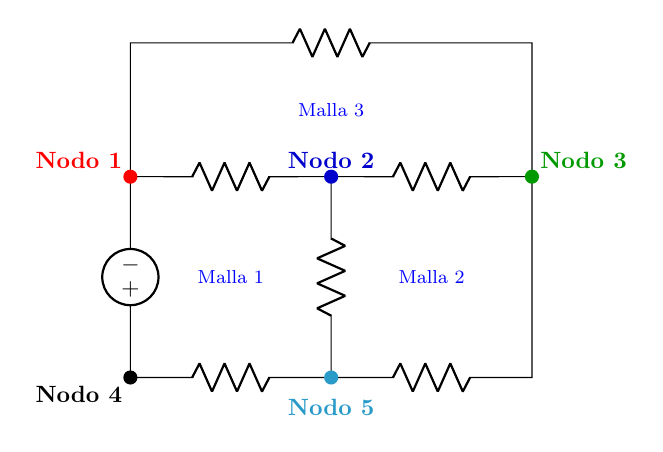
\begin{tikzpicture}[scale=0.85, transform shape]

        % 1. Tu circuito base intacto (Se dibuja siempre en negro)
        \draw (0,0) to[V] (0,3) to[R] (3,3) to[R] (6,3) -- (6,0) to[R] (3,0) to[R] (0,0);
        \draw (3,3) to[R] (3,0);
        \draw (0,3) -- (0,5) to[R] (6,5) -- (6,3);


        % 2. CAPA 1: MALLAS (Solo paso 1 en vivo, y siempre en handout)
        \uncover<2>{
            \node[blue] at (1.5,1.5) {\footnotesize{Malla 1}};

            \node[blue] at (4.5,1.5) {\footnotesize{Malla 2}};

            \node[blue] at (3,4) {\footnotesize{Malla 3}};
        }


        % 3. CAPA 2: NODOS (Solo paso 2 en vivo, y siempre en handout)
        \uncover<3>{
            \fill[red] (0,3) circle (3pt) node[above left, red] {\textbf{Nodo 1}};

            \fill[blue!80!black] (3,3) circle (3pt) node[above, blue!80!black] {\textbf{Nodo 2}};

            \fill[green!60!black] (6,3) circle (3pt) node[above right, green!60!black] {\textbf{Nodo 3}};

            \fill[cyan!80!black] (3,0) circle (3pt);
            \node[below, cyan!80!black] at (3,-0.2) {\textbf{Nodo 5}};

            \fill[black] (0,0) circle (3pt) node[below left, black] {\textbf{Nodo 4}};
        }

    \end{tikzpicture}
\end{frame}




% ==========================================
% SLIDE 3: LEYES DE CONSERVACIÓN (KIRCHHOFF)
% ==========================================
\begin{frame}{Leyes de Conservación (Kirchhoff)}
    \begin{columns}[T]
        \begin{column}{0.48\textwidth}
            \pause
            \begin{boxTeoria}{Ley de Corrientes (LCK)}
                \textbf{Principio:} Conservación de la carga.

                \vspace{0.2cm}
                En un nodo no se acumula carga neta:
                \[ \sum I_{\text{entran}} = \sum I_{\text{salen}} \]

                \vfill
                \footnotesize{\textit{Origen físico:} $\bm{\nabla} \cdot \bm{J} + \frac{\partial\rho}{\partial t} = 0$}
            \end{boxTeoria}
        \end{column}

        \begin{column}{0.48\textwidth}
            \pause
            \begin{boxTeoria}{Ley de Voltajes (LVK)}
                \textbf{Principio:} Conservación de la energía.

                \vspace{0.2cm}
                En una malla cerrada, el potencial eléctrico es conservativo:
                \[ \sum_{\text{malla}} \Delta V = 0 \]

                \vfill
                \footnotesize{\textit{Origen físico:} $\oint \bm{E} \cdot d\bm{\ell} \approx 0$}
            \end{boxTeoria}
        \end{column}
    \end{columns}
\end{frame}


% ==========================================
% SLIDE 4: DEDUCCIÓN DE RESISTORES EN SERIE
% ==========================================
\begin{frame}{Resistores en Serie}
    \begin{columns}[c]
        \begin{column}{0.45\textwidth}
            \pause
            \begin{center}
                \begin{circuitikz}[scale=0.85, transform shape]
                    \draw (0,0) node[left]{$A$} to[R, l_=$R_1$, o-*] (2.5,0) node[above]{$B$}
                    to[R, l_=$R_2$, *-o] (5,0) node[right]{$C$};
                    \draw[->, thick, blue!80!black] (0.5, 0.6) -- (1.5, 0.6) node[midway, above]{$I$};
                \end{circuitikz}
            \end{center}
        \end{column}
        \begin{column}{0.55\textwidth}
            \pause
            \textbf{Definición:} Dos elementos están en serie si comparten exclusivamente \textbf{un} nodo intermedio sin bifurcación extra.
            \pause
            \begin{enumerate}
                \item Por \textbf{LCK}: La corriente es idéntica en todos los elementos ($I_1 = I_2 = I$).
                \item Por \textbf{LVK}: $V_{AC} = V_1 + V_2$.
                \item Aplicando Ley de Ohm:
                      $$V_{AC} = I R_1 + I R_2 = I(R_1 + R_2)$$
            \end{enumerate}
            $$\mathbf{R_{\text{eq}} = R_1 + R_2 + \dots + R_n}$$

        \end{column}
    \end{columns}
\end{frame}

% ==========================================
% SLIDE 5: DEDUCCIÓN DE RESISTORES EN PARALELO
% ==========================================
\begin{frame}{Resistores en Paralelo}
    \begin{columns}[c]
        \begin{column}{0.45\textwidth}
            \pause
            \begin{center}
                \begin{circuitikz}[scale=0.85, transform shape]
                    \draw (0,1) node[left]{$A$} -- (1,1) -- (1,2) to[R=$R_1$] (3.5,2) -- (3.5,1) -- (4.5,1) node[right]{$B$};
                    \draw (1,1) -- (1,0) to[R=$R_2$] (3.5,0) -- (3.5,1);
                    \draw[->, thick, blue!80!black] (0.2, 1.3) -- (0.8, 1.3) node[midway, above]{$I_{\text{total}}$};
                \end{circuitikz}
            \end{center}
        \end{column}
        \begin{column}{0.55\textwidth}
            \pause
            \textbf{Definición:} Dos elementos están en paralelo si están conectados exactamente al mismo par de nodos.
            \pause
            \begin{enumerate}
                \item Por \textbf{LVK}: Misma caída de potencial ($V_1 = V_2 = V$).
                \item Por \textbf{LCK}: $I_{\text{total}} = I_1 + I_2$.
                \item Aplicando Ley de Ohm:
                      $$I_{\text{total}} = \frac{V}{R_1} + \frac{V}{R_2} = V\left(\frac{1}{R_1} + \frac{1}{R_2}\right)$$
            \end{enumerate}
            $$\mathbf{\frac{1}{R_{\text{eq}}} = \frac{1}{R_1} + \frac{1}{R_2} \implies R_{\text{eq}} = \frac{R_1 R_2}{R_1 + R_2}}$$
        \end{column}
    \end{columns}
\end{frame}

% ==========================================
% SLIDE 6: ESTRATEGIA DE RESOLUCIÓN
% ==========================================
\begin{frame}{Estrategia de Reducción y Amperímetro}
    \begin{boxTeoria}{Estrategia: "De afuera hacia adentro"}
        \pause
        \begin{enumerate}
            \item<+-> Identificar cada nodo independiente (o asignar un color/etiqueta).
            \item<+-> Localizar los terminales de la fuente de alimentación.
            \item<+-> Reducir asociaciones evidentes (serie/paralelo) desde el extremo más alejado hacia la fuente.
            \item<+-> Redibujar el circuito equivalente tras cada simplificación intermedia.
        \end{enumerate}
    \end{boxTeoria}
\end{frame}

% ==========================================
% SLIDE 7: PROBLEMA 1
% ==========================================
\begin{frame}{Problema 1}
    Determine la resistencia equivalente total vista por la fuente y calcule la corriente total registrada por el amperímetro.
    \begin{center}
        \begin{circuitikz}[scale=0.8, transform shape]
            % Parte fija inicial
            \draw (0,0) to[battery1, l=$60\,\text{V}$, invert] (0,3);

            % Solución real con modos de Beamer:
            % En modo presentacion aparece en la capa 1. En modo handout (impresión) NO se dibuja (capa 0).
            \uncover<1 | handout:0>{\draw (0,3) -- (2,3);}
            % En modo presentacion aparece en la capa 2+. En modo handout se fuerza a aparecer en la única hoja estática.
            \uncover<2->{\draw (0,3) to[ammeter, l=$3.048\,\text{A}$] (2,3);}

            % Resto del circuito fijo
            \draw (2,3) to[R=$12\,\Omega$] (4.5,3)
            to[R=$3\,\Omega$] (7.5,3)
            -- (8.5,3)
            to[R=$5\,\Omega$] (8.5,0)
            to[R=$6\,\Omega$] (4.5,0)
            to[R=$4\,\Omega$] (0,0);
            \draw (4.5,3) to[R=$5\,\Omega$, *-*] (4.5,0);
        \end{circuitikz}
    \end{center}
\end{frame}

% ==========================================
% SLIDE 8: PROBLEMA 2
% ==========================================
\begin{frame}{Problema 2}
    Determine la resistencia equivalente total vista por la fuente y compruebe la lectura del amperímetro.
    \begin{center}
        \begin{circuitikz}[scale=0.8, transform shape]
            \draw (0,0) to[battery1, l=$25\,\text{V}$, invert] (0,3);

            % Control estricto de capas y modo handout
            \uncover<1 | handout:0>{\draw (0,3) -- (4.5,3);}
            \uncover<2->{\draw (0,3) to[ammeter, l=$2.695\,\text{A}$] (4.5,3);}

            \draw (4.5,3) to[R=$3\,\Omega$] (8,3)
            to[R=$4\,\Omega$] (8,0)
            to[R=$2\,\Omega$] (6,0)
            to[R=$4\,\Omega$, *-*] (3,0)
            to[R=$6\,\Omega$] (0,0);
            \draw (4.5,3) to[R=$6\,\Omega$, *-*] (3,0);
            \draw (4.5,3) to[R=$5\,\Omega$, *-*] (6,0);
        \end{circuitikz}
    \end{center}
\end{frame}

% ==========================================
% SLIDE 9: PROBLEMA 3
% ==========================================
\begin{frame}{Problema 3}
    Calcule la resistencia equivalente total y verifique la corriente suministrada por la fuente de $75\,\text{V}$.
    \begin{center}
        \begin{circuitikz}[scale=0.8, transform shape]
            \draw (0,0) to[battery1, l=$75\,\text{V}$, invert] (0,2);

            % Control estricto de capas y modo handout
            \uncover<1 | handout:0>{\draw (0,2) -- (3,2);}
            \uncover<2->{\draw (0,2) to[ammeter, l=$7.471\,\text{A}$] (3,2);}

            \draw (0,0) to[R=$6\,\Omega$] (3,0);
            \draw (3,2) to[R=$6\,\Omega$, *-*] (3,0);
            \draw (3,2) to[R=$2\,\Omega$] (3,4)
            to[R=$4\,\Omega$] (8,4)
            to[R=$5\,\Omega$] (8,2);
            \draw (3,2) to[R=$3\,\Omega$] (8,2);
            \draw (8,2) to[R=$4\,\Omega$, *-] (8,0)
            to[R=$2\,\Omega$] (5.5,0)
            to[R=$4\,\Omega$] (3,0);
        \end{circuitikz}
    \end{center}
\end{frame}

\end{document}
